\section{\uppercase{Results}}

\subsection{Experiment 1}

\begin{figure}[!h]
  \vspace{-0.2cm}
  \centering
   {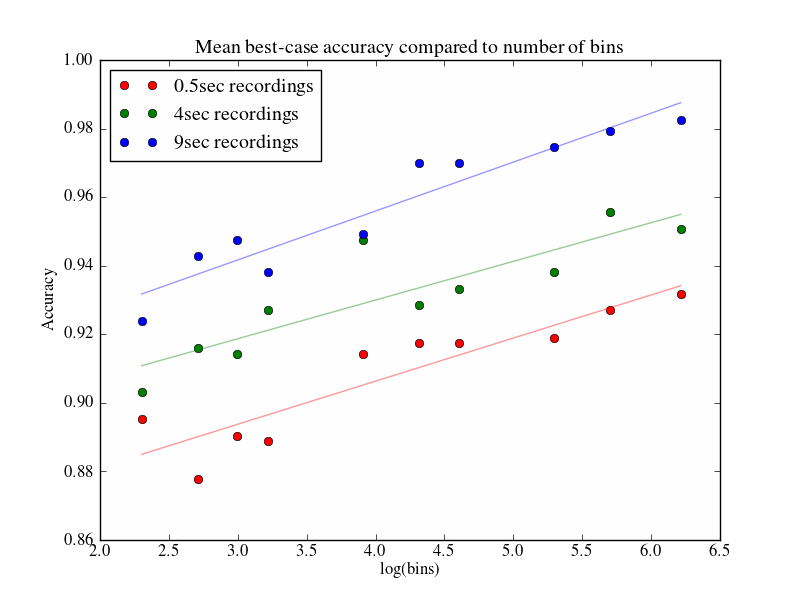
\epsfig{file = Figures/1-2.png, width = 5.5cm}}
  \caption{Mean best-case accuracy among all subjects compared to log of the number of bins in training data.}
  \label{fig:fig1}
  \vspace{-0.1cm}
 \end{figure}

Overall, both longer recording times and higher bin size are correlated with higher classifier accuracy. \textit{and what is important to report about this regression?}

\begin{figure}[!h]
  \vspace{-0.2cm}
  \centering
   {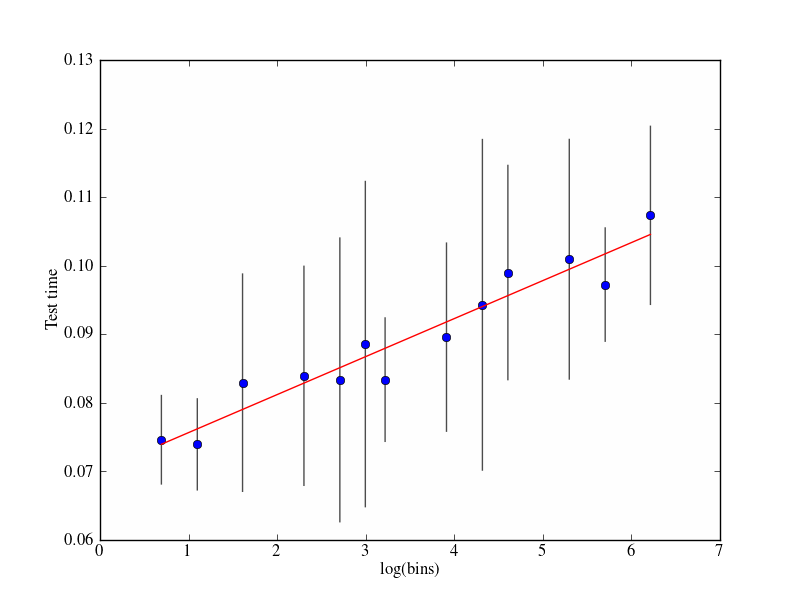
\epsfig{file = Figures/3-1.png, width = 5.5cm}}
  \caption{SVM test time compared to number of bins in test set feature vector.}
  \label{fig:fig2}
  \vspace{-0.1cm}
\end{figure}

\begin{figure}[!h]
  \vspace{-0.2cm}
  \centering
   {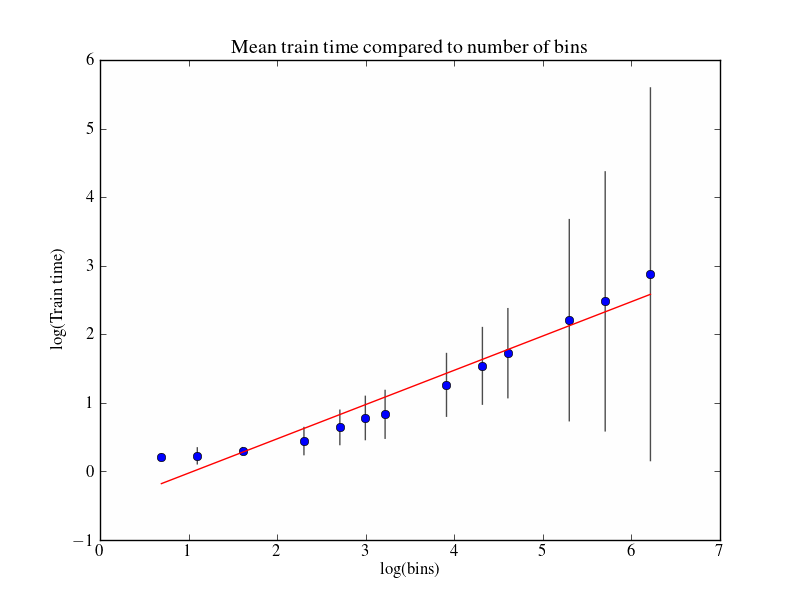
\epsfig{file = Figures/3.png, width = 5.5cm}}
  \caption{SVM train time compared to number of bins in training set feature vectors.}
  \label{fig:fig2}
  \vspace{-0.1cm}
\end{figure}


The number of bins is positively correlated with training and testing time. While test time grows linearly with the log of the number of bins, training time grows exponentially with the log of the number of bins. \textit{and what is important to report about this regression?}

\subsection{Experiment 2}

\begin{figure}[!h]
  \vspace{-0.2cm}
  \centering
   {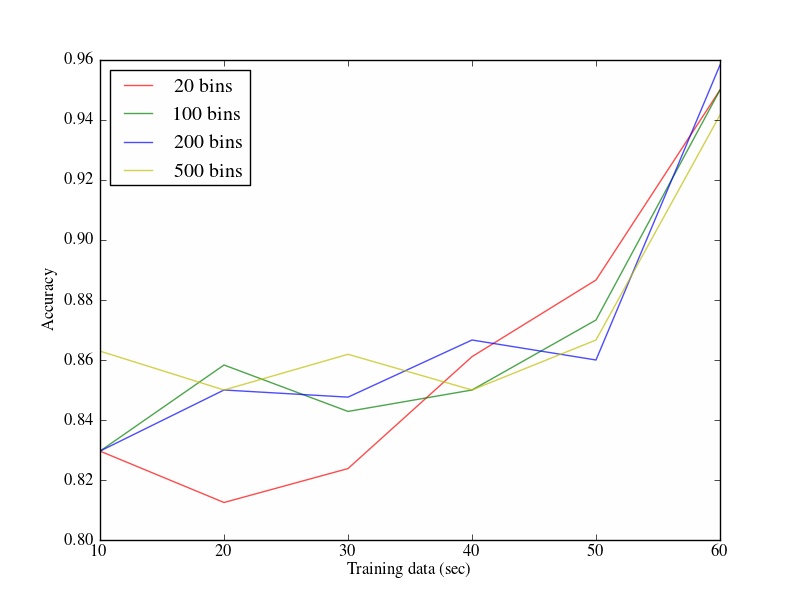
\epsfig{file = Figures/7.png, width = 5.5cm}}
  \caption{Mean best-case accuracy compared to number of seconds of data in training set.}
  \label{fig:fig2}
  \vspace{-0.1cm}
\end{figure}

 The amount of data on which the classifier is trained is positively correlated with the classifier's accuracy on data from later recordings. \textit{and what is important to report about this regression?}
